\StartOf{Lecture 9}

\Today{(0) Gaussan r.v.s from Lecture 8, (1) 1-D Detection }

\announcements{
\begin{itemize}
  \item Project 2 due today, 11:59pm.  HW 4 due Wednesday.
  \item Reading: today: Stephen M. Kay, ``Detection Theory'' Chapter 3.3 \& 3.6 (pdf on Canvas).  Wed: Rice 4.4-4.5
\end{itemize}
}

\section{Bayesian 1-D Detection}

When we say `optimal detection' in the Bayesian detection framework,
we mean that we want the smallest probability of error.  The
probability of error is denoted
\[
  \PR{\mbox{symbol error}}
\]
By error, we mean that a different symbol was detected than the symbol
that was sent.   At the start of every detection problem, we list the
events that could have occurred, \ie, the symbols that could have
been sent. We follow all detection and statistics textbooks and label these classes $H_i$.

Later we will use detection theory to describe why we use a matched filter.  For now, we're studying a somewhat simpler problem, assuming that our receiver uses a matched filter, time synchronization block, and downsampling block.
Our receivers need to make a decision after the downsampling. based on the voltages $X_i$ measured at this point, for each waveform $\phi_i(t)$.  Further for this lecture, we are studying the case when there is only one waveform, e.g., PAM.  Thus we call this voltage $X$ for simplicity.  The voltage $X$ should be close to one of $M$ possible symbol values $a_0, \ldots, a_{M-1}$.  

In summary we describe the decision as a list of \emph{models} that describe what the conditional distribution of $X$ is given that the $i$th symbol is sent:
\begin{eqnarray}
  H_0: && X = a_0 + W \nonumber \\
  H_1: && X = a_1 + W \nonumber \\
  \cdots && \cdots \nonumber \\
  H_{M-1}: && X = a_{M-1} + W \nonumber
\end{eqnarray}
where $W$ is Gaussian additive noise with mean 0 and variance $\sigma^2$.
This must be a complete listing of events.  That is, the events $H_0
\cup H_1 \cup \cdots \cup H_{M-1} = S$, where the $\cup$ means
union, and $S$ is the complete event space.



Let's just say for now that there are only two symbols, i.e., $M=2$.  We
need to decide from $X$ whether symbol 0 or symbol 1 was sent.

The hypotheses are:
\begin{eqnarray}
  H_0: && X = a_0 + W \nonumber \\
  H_1: && X = a_1 + W \nonumber
\end{eqnarray}  % pause.

We use the law of total probability to say that
\begin{eqnarray}
  \PR{\mbox{error}}    &=& \PR{\mbox{error} \cap H_0} +  \PR{\mbox{error} \cap H_1 }
\end{eqnarray}
Where the cap means `and'. Then using Bayes' Law,
\[
   \PR{\mbox{error}}  = \PR{\mbox{error} | H_0}\PR{H_0} +  \PR{\mbox{error} | H_1 }\PR{H_1}
\]

\subsection{Decision Region}

We're making a decision based only on $X$.  Over some set $R_0$ of
values of $X$, we'll decide that $H_0$ happened (symbol 0 was sent).
Over a different set $R_1$ of values, we'll decide $H_1$ occurred
(that symbol 1 was sent).  \emph{We can't be indecisive}, so
\begin{itemize}
  \item There is no overlap: $R_0 \cap R_1 = \emptyset$.
  \item There are no values of $x$ disregarded: $R_0 \cup R_1 = S$.
\end{itemize}

\subsection{Formula for Probability of Error}

So the probability of error is
\begin{equation} \label{E:PeBayesianBasic}
   \PR{\mbox{error}}  = \PR{X \in R_1 | H_0}\PR{H_0} +  \PR{X \in R_0 | H_1 }\PR{H_1}
\end{equation}
The probability that $X$ is in $R_1$ is one minus the probability
that it is in $R_0$, since the two are complementary sets.
\begin{eqnarray}
   \PR{\mbox{error}}  &=& (1 - \PR{X \in R_0 | H_0} )\PR{H_0} +  \PR{X \in R_0 | H_1 }\PR{H_1}
     \nonumber \\
   \PR{\mbox{error}}  &=& \PR{H_0} - \PR{X \in R_0 | H_0} \PR{H_0} +  \PR{X \in R_0 | H_1 }\PR{H_1}
     \nonumber
\end{eqnarray}
Now note that probabilities that $X \in R_0$ are integrals over the
 event (region) $R_0$.
\begin{eqnarray}
   \PR{\mbox{error}}  &=& \PR{H_0} - \int_{x \in R_0} f_{X|H_0}(x| H_0) \PR{H_0}
   dx \nnn
     &&                             +  \int_{x \in R_0} f_{X|H_1}(x | H_1) \PR{H_1} dx
     \nonumber \\
     &=& \PR{H_0} +     \label{E:PeAsAFcnOfR1} \\
     && \int_{x \in R_0} \left\{f_{X|H_1}(x | H_1) \PR{H_1} - f_{X|H_0}(x| H_0) \PR{H_0} \right\}
     dx \nn
\end{eqnarray}
We've got a lot of things in the expression in
(\ref{E:PeAsAFcnOfR1}), but the only thing we can change is the
region $R_0$.  Everything else is determined by the time we get to
this point.  So the question is, how do you pick $R_0$ to minimize
(\ref{E:PeAsAFcnOfR1})?

\subsection{Selecting $R_0$ to Minimize Probability of Error}

We can see what the integrand looks like.  Figure
\ref{F:plotLikelihoodFunctionsBinaryRx}(a) shows the conditional
probability density functions.  Figure \ref{F:plotLikelihoodFunctionsBinaryRx}(b)
shows the joint densities (the conditional pdfs multiplied by the
bit probabilities $\PR{H_0}$ and $\PR{H_1}$.  Finally, Figure
\ref{F:plotLikelihoodFunctionsBinaryRx}(c) shows the full integrand of
(\ref{E:PeAsAFcnOfR1}), the difference between the joint densities.
\begin{figure}[htbp]
  \centerline{(a) \includegraphics[width=3in]{../images/plotLikelihoodFunctionsBinaryRx.eps}}
  \centerline{(b) 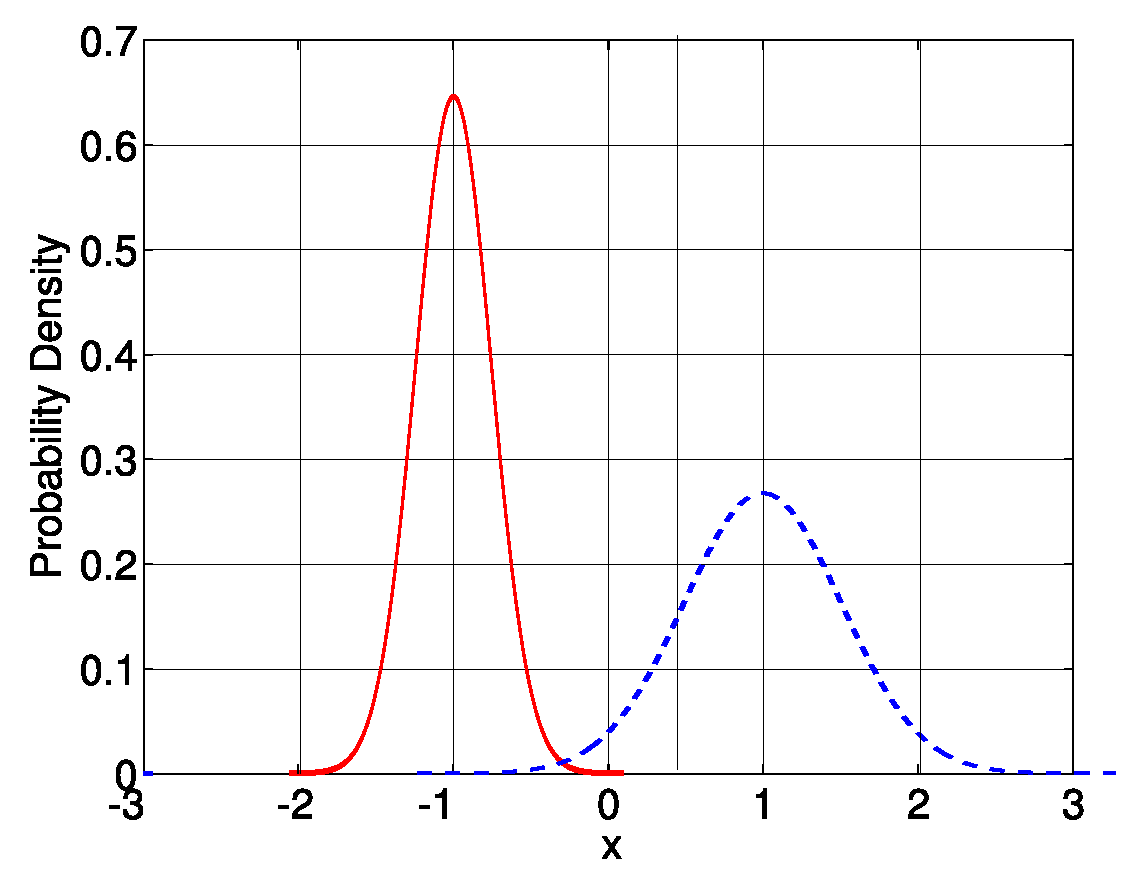
\includegraphics[width=3in]{../images/plotJointDensities.eps}}
  \centerline{(c) \includegraphics[width=3in]{../images/plotJointDensityDifference.eps}}
  \caption{The (a) conditional p.d.f.s (likelihood functions) $f_{X|H_0}(x|H_0)$ and $f_{X|H_1}(x|H_1)$, (b) joint p.d.f.s $f_{X|H_0}(x|H_0)\PR{H_0}$ and $f_{X|H_1}(x|H_1)\PR{H_1}$, and (c) difference between the joint p.d.f.s,
  $f_{X|H_1}(x|H_1)\PR{H_1} - f_{X|H_0}(x|H_0)\PR{H_0}$,
  which is the integrand in (\ref{E:PeAsAFcnOfR1}).}
  \label{F:plotLikelihoodFunctionsBinaryRx}
\end{figure}
% \begin{figure}[hp]
%   \caption{The joint p.d.f.s $f_{X|H_0}(x|H_0)\PR{H_0}$ and $f_{X|H_1}(x|H_1)\PR{H_1}$.}
%   \label{F:plotJointDensities}
% \end{figure}
% \begin{figure}[hp]
%   \caption{The difference between the joint p.d.f.s,
%   $f_{X|H_1}(x|H_1)\PR{H_1} - f_{X|H_0}(x|H_0)\PR{H_0}$,
%   which is the integrand in (\ref{E:PeAsAFcnOfR1}).}
%   \label{F:plotJointDensityDifference}
% \end{figure}

We can pick $R_0$ however we want - we just say what region of $x$,
and the integral in (\ref{E:PeAsAFcnOfR1}) will integrate over it.
The objective is to minimize the probability of error.  Which $x$'s
should we include in the region?  Should we include $x$ which has a
positive value of the integrand?  Or should we include the parts of
$x$ which have a negative value of the integrand?

\Solution{Select $R_0$ to be all $x$ such that the integrand is
negative.}

Then $R_0$ is the area in which
\[
  f_{X|H_0}(x|H_0) \PR{H_0} > f_{X|H_1}(x|H_1) \PR{H_1}
\]
If $\PR{H_0} = \PR{H_1}$, then this is the region in which $X$ is
more probable given $H_0$ than given $H_1$.

Rearranging the terms,
\begin{equation} \label{E:BayesianLikelihoodRatio}
  \frac{f_{X|H_1}(x|H_1)}{f_{X|H_0}(x|H_0)}  < \frac{\PR{H_0}}{ \PR{H_1}}
\end{equation}
The left hand side is called the likelihood ratio.  The right hand
side is a threshold.  Whenever $x$ indicates that the likelihood
ratio is less than the threshold, then we'll decide $H_0$, \ie, that
$s_0(t)$ was sent.  Otherwise, we'll decide $H_1$, \ie, that
$s_1(t)$ was sent.

Equation (\ref{E:BayesianLikelihoodRatio}) is a very general result,
applicable no matter what conditional distributions $x$ has.

\subsection{Log-Likelihood Ratio}

For the Gaussian distribution, the math gets much easier if we take
the log of both sides.  Why can we do this?

\Solution{ 1.  Both sides are positive, 2. The $\log()$ function is
strictly increasing.}

Now, the \emph{log-likelihood ratio} is
\[
  \log \frac{f_{X|H_1}(x|H_1)}{f_{X|H_0}(x|H_0)}  < \log \frac{\PR{H_0}}{ \PR{H_1}}
\]

\subsection{Case of $a_0 = 0$, $a_1 = 1$ in Gaussian noise}

In this example, $W \sim \mathcal{N}(0,\sigma_w^2)$.  In addition,
assume for a minute that $a_0 = 0$ and $a_1 = 1$.  What is:
\begin{enumerate}
  \item The log of a Gaussian pdf?
  \item The log-likelihood ratio?
  \item The decision regions for $x$?
\end{enumerate}

\Solution{ What is the log of a Gaussian pdf?
\begin{eqnarray}
 \log f_{X|H_0}(x|H_0) &=& \log \left[ \frac{1}{\sqrt{2\pi \sigma_w^2}} e^{-\frac{x^2}{2\sigma_w^2}} \right]
   \nonumber \\
 &=& -\frac{1}{2}\log (2\pi \sigma_w^2)  - \frac{x^2}{2\sigma_w^2}
\end{eqnarray}
The $\log f_{X|H_1}(x|H_1)$ term will be the same but with
$(x-1)^2$instead of $x^2$. Continuing with the log-likelihood ratio,
\begin{eqnarray}
   \log f_{X|H_1}(x|H_1) - \log f_{X|H_0}(x|H_0)  &<& \log \frac{\PR{H_0}}{ \PR{H_1}} \nonumber \\
   \frac{x^2}{2\sigma_w^2} - \frac{(x-1)^2}{2\sigma_w^2}  &<& \log \frac{\PR{H_0}}{ \PR{H_1}} \nonumber \\
   x^2 - (x-1)^2  &<& 2\sigma_w^2 \log \frac{\PR{H_0}}{ \PR{H_1}} \nonumber \\
   2x - 1  &<& 2\sigma_w^2 \log \frac{\PR{H_0}}{ \PR{H_1}} \nonumber \\
   x  &<& \frac{1}{2} + \sigma_w^2 \log \frac{  \PR{H_0}}{ \PR{H_1}} \nonumber
\end{eqnarray}
}

In the end result, there is a simple test for $x$ - if it is below
the \emph{decision threshold}, decide $H_0$.  If it is above the
decision threshold,
\[
x  > \frac{1}{2} + \sigma_w^2 \log \frac{  \PR{H_0}}{ \PR{H_1}}
\]
decide $H_1$.  Rather than writing both inequalities each time, we
use the following notation:
\[
 x  \decision{H_1}{H_0} \frac{1}{2} + \sigma_w^2 \log \frac{  \PR{H_0}}{\PR{H_1}}
\]
This completely describes the detector receiver.

For simplicity, we also write $x  \decision{H_1}{H_0} \gamma$ where
\begin{equation} \label{E:decisionThreshold}
  \gamma = \frac{1}{2} + \sigma_w^2 \log \frac{  \PR{H_0}}{\PR{H_1}}
\end{equation}

\subsection{General Case for Arbitrary Symbols}

If, instead of $a_0 = 0$ and $a_1 = 1$, we had arbitrary values for
them (the signal space representations of $s_0(t)$ and $s_1(t)$), we
could have derived the result in the last section the same way.  As
long as $a_0 < a_1$, we'd still have $r \decision{H_1}{H_0} \gamma$,
but now,
\begin{equation} \label{E:decisionThresholdGeneral}
  \gamma = \frac{a_0 + a_1}{2} + \frac{\sigma_w^2}{a_1 - a_0} \log \frac{  \PR{H_0}}{\PR{H_1}}
\end{equation}

\subsection{Equi-probable Special Case}

If symbols are equally likely, $\PR{H_1} = \PR{H_0}$, then
$\frac{\PR{H_1}}{  \PR{H_0}} = 1$ and the logarithm of the fraction
is zero.  So then
\[
 x  \decision{H_1}{H_0} \frac{a_0 + a_1}{2}
\]
The decision above says that if $x$ is closer to $a_0$, decide that
$s_0(t)$ was sent. And if $x$ is closer to $a_1$, decide that
$s_1(t)$ was sent. The boundary is exactly half-way in between the
two signal space vectors.

This receiver is also called a maximum likelihood detector, because
we only decide which likelihood function is higher (neither is
scaled by the prior probabilities $\PR{H_0}$ or $\PR{H_1}$.

\subsection{Examples}

\Example{When $H_1$ becomes less likely, which direction will the
optimal threshold move, towards $a_0$ or towards $a_1$?}

\Solution{Towards $a_1$.}

\Example{Let $a_0 = -1$, $a_1 = 1$, $\sigma_w^2 = 0.1$, $\PR{H_1} =
0.4$, and $\PR{H_0}=0.6$.  What is the decision threshold for $x$?}

\Solution{ From (\ref{E:decisionThresholdGeneral}),
\[
  \gamma = 0 + \frac{0.1}{2} \log \frac{0.6}{0.4} = 0.05 \log 1.5
  \approx 0.0203
\]
}

\Example{Can the decision threshold be higher than both $a_0$ and
$a_1$ in this binary, one-dimensional modulation, receiver?}

\Solution{Yes, it can.  You can make $\log \frac{  \PR{H_0}}{\PR{H_1}}$ arbitrarily high, try it!}

Given $a_0$, $a_1$, $\sigma_w^2$, $\PR{H_1}$, and $\PR{H_0}$, you
should be able to calculate the optimal decision threshold $\gamma$.

\Example{In this example, given all of the above constants and the optimal threshold $\gamma$,
calculate the probability of error from (\ref{E:PeBayesianBasic}).}
Starting from
\[
   \PR{\mbox{error}}  = \PR{x \in R_1 | H_0}\PR{H_0} +  \PR{x \in R_0 | H_1 }\PR{H_1}
\]
we can use the decision regions in (\ref{E:decisionThreshold}) to
write
\[
   \PR{\mbox{error}}  = \PR{x > \gamma | H_0}\PR{H_0} +  \PR{x < \gamma | H_1 }\PR{H_1}
\]
What is the first probability, given that $r|H_0$ is Gaussian with
mean $a_0$ and variance $\sigma_w^2$?  What is the second
probability, given that $x|H_1$ is Gaussian with mean $a_1$ and
variance $\sigma_w^2$?  What is then the overall probability of
error?

\Solution{
\begin{eqnarray}
  \PR{x > \gamma | H_0} &=& \Q{ \frac{\gamma - a_0}{\sigma_w} }
    \nonumber \\
  \PR{x < \gamma | H_1} &=& 1 - \Q{ \frac{\gamma - a_1}{\sigma_w} }
    = \Q{ \frac{a_1 - \gamma}{\sigma_w} }
    \nonumber \\
  \PR{\mbox{error}}  &=& \PR{H_0} \Q{ \frac{\gamma - a_0}{\sigma_w} } +
    \PR{H_1}\Q{ \frac{a_1 - \gamma}{\sigma_w} } \nonumber
\end{eqnarray}
}


\subsection{Review of Binary Detection}
We did three things to prove some things about the optimal detector:
\begin{itemize}
  \item We wrote the formula for the probability of error.
  \item We found the decision regions which minimized the probability of error.
  \item We used the log operator to show that for the Gaussian error case the decision regions are separated by a single threshold.
  \item We showed the formula for that threshold, both in the equi-probable symbol case, and in the general case.
\end{itemize}
